\documentclass{article}
\usepackage{amsmath, graphicx, hyperref, listings, float, caption, geometry}
\geometry{margin=1in}

\title{AMS 595 - Assignment 4: Fractal Approximation}
\author{Amol Arora, SBUID: 116491705}
\date{\today}

\begin{document}

\maketitle

\section{Introduction}
This project involves implementing three computational tasks in Python: generating the Mandelbrot set, simulating a Markov chain, and approximating functions using Taylor series expansions. The primary objectives are to explore fractal generation, observe long-term behavior in stochastic systems, and approximate complex functions using polynomial expansions. Each task leverages different mathematical concepts, reinforcing practical programming skills and analytical techniques.

\section{Methodology}

\subsection{Mandelbrot Set}
The goal for this task was to create a Python script, \texttt{mandelbrot.py}, that calculates and visualizes the Mandelbrot set. The set is defined by the recursive relation:
\[
z_{n+1} = z_n^2 + c, \quad z_0 = 0
\]
where a complex number \(c\) belongs to the Mandelbrot set if the iteration remains bounded. For this implementation:
\begin{itemize}
    \item A grid of complex numbers \(c\) was created over the range \([-2, 1] \times [-1.5, 1.5]\).
    \item A threshold of 50 iterations was used to assess divergence.
    \item Using the \texttt{numpy.mgrid} function, a 500x500 grid was constructed, and divergence was checked by maintaining a mask array.
\end{itemize}
The final output was an image of the Mandelbrot fractal, generated using \texttt{matplotlib}. Project code for this implementation is shown below:
\begin{lstlisting}[language=Python]
import numpy as np
import matplotlib.pyplot as plt

def mandelbrot(threshold=50):
    x, y = np.mgrid[-2:1:500j, -1.5:1.5:500j]
    c = x + 1j * y
    z = np.zeros_like(c, dtype=complex)
    mask = np.full(c.shape, True, dtype=bool)

    for i in range(threshold):
        z[mask] = z[mask]**2 + c[mask]
        mask = mask & (np.abs(z) < 100)
    
    plt.imshow(mask.T, extent=[-2, 1, -1.5, 1.5])
    plt.gray()
    plt.savefig('mandelbrot.png')
    plt.show()

mandelbrot()
\end{lstlisting}

\subsection{Markov Chain}
This part required a script, \texttt{markov\_chain.py}, that simulates a Markov chain with 5 states. The main steps were:
\begin{itemize}
    \item Generating a random 5x5 transition matrix and normalizing rows to ensure each row summed to 1.
    \item Constructing a random initial probability vector and applying the transition rule 50 times.
    \item Computing the stationary distribution by finding the eigenvector associated with eigenvalue 1 of the transition matrix \(P^T\).
\end{itemize}
The script outputted the stationary distribution and confirmed convergence within a tolerance of \(10^{-5}\). Key code snippets are provided below:
\begin{lstlisting}[language=Python]
import numpy as np

P = np.random.rand(5, 5)
P = P / P.sum(axis=1, keepdims=True)
p = np.random.rand(5)
p /= p.sum()

for _ in range(50):
    p = P.T @ p

eigenvalues, eigenvectors = np.linalg.eig(P.T)
stationary = eigenvectors[:, np.isclose(eigenvalues, 1)]
stationary = stationary / stationary.sum()

diff = np.abs(p - stationary.flatten())
print("Difference within tolerance:", np.all(diff < 1e-5))
\end{lstlisting}

\subsection{Taylor Series Approximation}
The task here was to write a script, \texttt{taylor.py}, that approximates the function \( f(x) = x \sin^2(x) + \cos(x) \) over the interval \([-10, 10]\) using a Taylor series expansion with up to 100 terms. We calculated the Taylor series at \( c = 0 \) using SymPy, and stored error and runtime data for different degrees in a CSV file.
\begin{itemize}
    \item SymPy was used to compute derivatives, allowing for a truncated series up to a specified degree.
    \item The error and computation time for each approximation degree were saved to \texttt{taylor\_values.csv}.
\end{itemize}
\begin{lstlisting}[language=Python]
import numpy as np
import pandas as pd
import sympy as sp
import time
import matplotlib.pyplot as plt

def taylor_approx(func, start, end, degree, c):
    x = sp.symbols('x')
    f = func(x)
    taylor_series = sum(f.diff(x, n).subs(x, c) * (x - c)**n / sp.factorial(n) for n in range(degree + 1))
    f_approx = sp.lambdify(x, taylor_series, 'numpy')
    x_vals = np.linspace(start, end, 100)
    return f_approx(x_vals), x_vals
\end{lstlisting}

\section{Results}

\subsection{Mandelbrot Set}
The resulting image of the Mandelbrot fractal is shown below:
\begin{figure}[H]
    \centering
    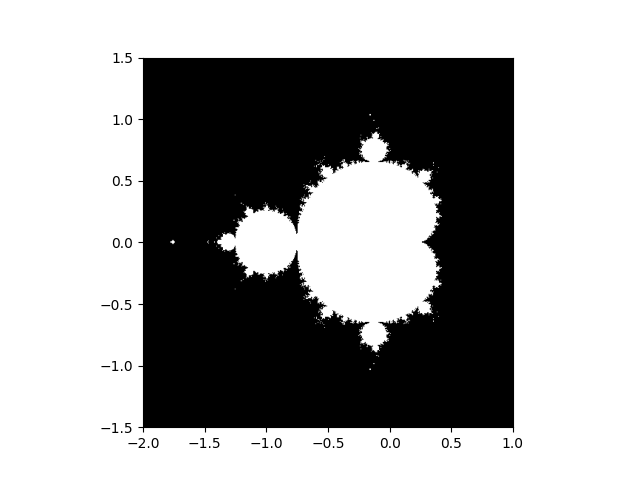
\includegraphics[width=0.6\textwidth]{C:/Users/amoarora/OneDrive - Stony Brook University/Desktop/595-Assignment/results/mandelbrot.png}
    \caption{Generated Mandelbrot Set}
\end{figure}

\subsection{Markov Chain}
The stationary distribution was found and matched closely with the 50-step distribution within the specified tolerance. This supports the theoretical convergence of Markov chains to a stationary distribution under the conditions met.

\subsection{Taylor Series Approximation}
The approximation of \( f(x) = x \sin^2(x) + \cos(x) \) showed high accuracy near the expansion point \( c = 0 \), with divergence observed near the interval edges. Below is a plot comparing the original function with its Taylor series approximation:
\begin{figure}[H]
    \centering
    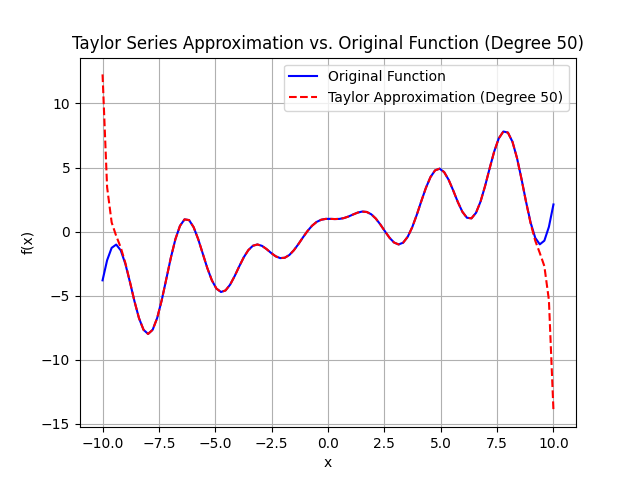
\includegraphics[width=0.6\textwidth]{C:/Users/amoarora/OneDrive - Stony Brook University/Desktop/595-Assignment/results/taylor_approximation.png}
    \caption{Taylor Series Approximation vs. Original Function}
\end{figure}

\section{Discussion}
The Mandelbrot fractal demonstrates the complex behavior of iterated functions in the complex plane. The Markov chain simulation verified convergence to a stationary distribution, aligning with theoretical expectations. The Taylor series approximation effectively matched the target function near \( c = 0 \), but diverged at the interval edges due to the polynomial nature of Taylor expansions. The project highlights practical implementations of mathematical concepts and the importance of convergence considerations in numerical approximations.

\end{document}
